%%%%%%%%%%%%%%%%%%%%%%%%%%%%%%%%%%%%%%%%%
% Beamer Presentation
% LaTeX Template
% Version 1.0 (10/11/12)
%
% This template has been downloaded from:
% http://www.LaTeXTemplates.com
%
% License:
% CC BY-NC-SA 3.0 (http://creativecommons.org/licenses/by-nc-sa/3.0/)
%
%%%%%%%%%%%%%%%%%%%%%%%%%%%%%%%%%%%%%%%%%

%----------------------------------------------------------------------------------------
%	PACKAGES AND THEMES
%----------------------------------------------------------------------------------------

\documentclass{beamer}

\mode<presentation> {

% The Beamer class comes with a number of default slide themes
% which change the colors and layouts of slides. Below this is a list
% of all the themes, uncomment each in turn to see what they look like.

% \usetheme{default}
%\usetheme{AnnArbor}
%\usetheme{Antibes}
% \usetheme{Bergen}
%\usetheme{Berkeley}
%\usetheme{Berlin}
%\usetheme{Boadilla}
% \usetheme{CambridgeUS}
%\usetheme{Copenhagen}
%\usetheme{Darmstadt}
%\usetheme{Dresden}
% \usetheme{Frankfurt}
%\usetheme{Goettingen}
%\usetheme{Hannover}
%\usetheme{Ilmenau}
%\usetheme{JuanLesPins}
%\usetheme{Luebeck}
\usetheme{Madrid}
%\usetheme{Malmoe}
%\usetheme{Marburg}
%\usetheme{Montpellier}
%\usetheme{PaloAlto}
%\usetheme{Pittsburgh}
%\usetheme{Rochester}
%\usetheme{Singapore}
%\usetheme{Szeged}
%\usetheme{Warsaw}

% As well as themes, the Beamer class has a number of color themes
% for any slide theme. Uncomment each of these in turn to see how it
% changes the colors of your current slide theme.

%\usecolortheme{albatross}
%\usecolortheme{beaver}
%\usecolortheme{beetle}
%\usecolortheme{crane}
%\usecolortheme{dolphin}
%\usecolortheme{dove}
%\usecolortheme{fly}
%\usecolortheme{lily}
%\usecolortheme{orchid}
%\usecolortheme{rose}
%\usecolortheme{seagull}
%\usecolortheme{seahorse}
%\usecolortheme{whale}
%\usecolortheme{wolverine}

%\setbeamertemplate{footline} % To remove the footer line in all slides uncomment this line
%\setbeamertemplate{footline}[page number] % To replace the footer line in all slides with a simple slide count uncomment this line

%\setbeamertemplate{navigation symbols}{} % To remove the navigation symbols from the bottom of all slides uncomment this line
}

\usepackage{graphicx} % Allows including images
\usepackage{booktabs} % Allows the use of \toprule, \midrule and \bottomrule in tables
\usepackage{listings}

\lstdefinestyle{customjava}{
  breaklines=true,
  frame=L,
  xleftmargin=\parindent,
  language=Java,
  showstringspaces=false,
  basicstyle=\footnotesize\ttfamily,
  keywordstyle=\bfseries\color{green!40!black},
  commentstyle=\itshape\color{gray!40!black},
  identifierstyle=\color{blue},
  stringstyle=\color{orange},
}
%----------------------------------------------------------------------------------------
%	TITLE PAGE
%----------------------------------------------------------------------------------------

\title[Programming 2]{Programming 2 Revision} % The short title appears at the bottom of every slide, the full title is only on the title page

\author{Jonathan Windle} % Your name
\institute[UEA] % Your institution as it will appear on the bottom of every slide, may be shorthand to save space
{
University of East Anglia \\ % Your institution for the title page
\medskip
\textit{J.Windle@uea.ac.uk} % Your email address
}
\date{\today} % Date, can be changed to a custom date7

\begin{document}

\begin{frame}
\titlepage % Print the title page as the first slide
\end{frame}

\begin{frame}[allowframebreaks]
\frametitle{Overview} % Table of contents slide, comment this block out to remove it
\tableofcontents % Throughout your presentation, if you choose to use \section{} and \subsection{} commands, these will automatically be printed on this slide as an overview of your presentation
\end{frame}

%----------------------------------------------------------------------------------------
%	PRESENTATION SLIDES
%----------------------------------------------------------------------------------------

%------------------------------------------------
\section{Threads} % Sections can be created in order to organize your presentation into discrete blocks, all sections and subsections are automatically printed in the table of contents as an overview of the talk
%------------------------------------------------

\subsection{Parallel structures} % A subsection can be created just before a set of slides with a common theme to further break down your presentation into chunks

% \begin{frame}
% \frametitle{Paragraphs of Text}
% Sed iaculis dapibus gravida. Morbi sed tortor erat, nec interdum arcu. Sed id lorem lectus. Quisque viverra augue id sem ornare non aliquam nibh tristique. Aenean in ligula nisl. Nulla sed tellus ipsum. Donec vestibulum ligula non lorem vulputate fermentum accumsan neque mollis.\\~\\

% Sed diam enim, sagittis nec condimentum sit amet, ullamcorper sit amet libero. Aliquam vel dui orci, a porta odio. Nullam id suscipit ipsum. Aenean lobortis commodo sem, ut commodo leo gravida vitae. Pellentesque vehicula ante iaculis arcu pretium rutrum eget sit amet purus. Integer ornare nulla quis neque ultrices lobortis. Vestibulum ultrices tincidunt libero, quis commodo erat ullamcorper id.
% \end{frame}

%------------------------------------------------

% \begin{frame}
% \frametitle{Bullet Points}
% \begin{itemize}
% \item Lorem ipsum dolor sit amet, consectetur adipiscing elit
% \item Aliquam blandit faucibus nisi, sit amet dapibus enim tempus eu
% \item Nulla commodo, erat quis gravida posuere, elit lacus lobortis est, quis porttitor odio mauris at libero
% \item Nam cursus est eget velit posuere pellentesque
% \item Vestibulum faucibus velit a augue condimentum quis convallis nulla gravida
% \end{itemize}
% \end{frame}

%------------------------------------------------

% \begin{frame}
% \frametitle{Blocks of Highlighted Text}
% \begin{block}{Block 1}
% Lorem ipsum dolor sit amet, consectetur adipiscing elit. Integer lectus nisl, ultricies in feugiat rutrum, porttitor sit amet augue. Aliquam ut tortor mauris. Sed volutpat ante purus, quis accumsan dolor.
% \end{block}

% \begin{block}{Block 2}
% Pellentesque sed tellus purus. Class aptent taciti sociosqu ad litora torquent per conubia nostra, per inceptos himenaeos. Vestibulum quis magna at risus dictum tempor eu vitae velit.
% \end{block}

% \begin{block}{Block 3}
% Suspendisse tincidunt sagittis gravida. Curabitur condimentum, enim sed venenatis rutrum, ipsum neque consectetur orci, sed blandit justo nisi ac lacus.
% \end{block}
% \end{frame}

%------------------------------------------------

\begin{frame}
\frametitle{Parallel Structures}
\fontsize{8pt}{7.2}
\begin{columns}[t] % The "c" option specifies centered vertical alignment while the "t" option is used for top vertical alignment

\column{.33\textwidth} % Left column and width
\textbf{Shared Memory}
\begin{itemize}
\item Different processes access the same memory concurrently
\item Each \textbf{process} shares memory with other \textbf{processes}.
\item Structure adopted by multi core PC units now commonly available.
\end{itemize}
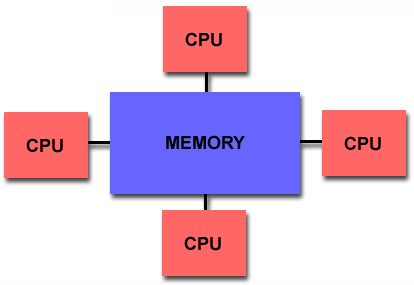
\includegraphics[width =\textwidth]{shared_mem.jpg}

\column{.33\textwidth} % Right column and width
\textbf{Distributed Memory}
\begin{itemize}
\item Each CPU has its own memory.
\item Messages passed between processes to coordinate their output.
\item Structure adopted by High-Performance Computing (HPC) facilities.
\end{itemize}
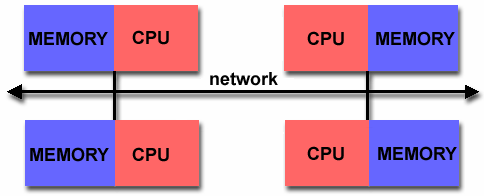
\includegraphics[width =\textwidth]{dist_mem.png}

\column{.33\textwidth}
\textbf{Combined Shared/Distributed Memory}
\begin{itemize}
\item Some CPUs share memory, some communicate via messages.
\item Local processes also communicate with other groups via messaging.
\end{itemize}
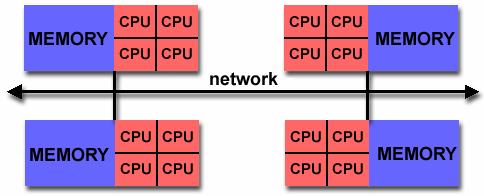
\includegraphics[width =\textwidth]{com_shared.png}

\end{columns}
\end{frame}

%------------------------------------------------
\subsection{Processes \& Threads}
%------------------------------------------------

\begin{frame}
\frametitle{Processes \& Threads}
\begin{itemize}
\item When program is launched, a {\color{red}process} is created.
\item {\color{red} Processes} can be sent to different processors by message passing scheme.
\item A {\color{green} thread} is a {\color{blue} portion} of a {\color{red} process} that can run {\color{blue} independently and concurrently} with other portions of the {\color{red} process}.
\item {\color{green} Threads} within a {\color{red} process} can share data.
\item {\color{green} Threads} rely on the OS (or other program) to determine what processor they are sent to.
\end{itemize}
\end{frame}

%------------------------------------------------
\subsection{Concurrent Programming}
\begin{frame}
\frametitle{Concurrent Programming}
\begin{itemize}
\item Involves development of algorithms for running {\color{red}simultaneously} in {\color{red}multiple threads}.
\item Java is inherently concurrent (Basic specification allows concurrent code development).
\item C++ needs special library (e.g. pthreads) {\color{blue}C\# is threaded}.
\item Java does not allow for user controlled parallel processing.
\end{itemize}
\end{frame}

%------------------------------------------------
\subsection{Java Threads}
\subsubsection{overview}
\begin{frame}[fragile] % Need to use the fragile option when verbatim is used in the slide
\frametitle{Overview}
\begin{itemize}
\item Any Java program has at least one thread, {\color{red}main}.
\item Any Java thread of execution is associated with an {\color{blue}instance} of the {\color{green} Thread} class.
\item Before new thread can start, a new instance of the {\color{green} Thread} class must be {\color{blue}instantiated}.
\item A java thread class implements the {\color{purple} Runnable} interface. Therefore every {\color{green} Thread} instance has a method:
\end{itemize}
\defverbatim[colored]\lstI{
\begin{lstlisting}[style = customjava,basicstyle=\ttfamily]
public void run() {...}
\end{lstlisting}
}
\lstI
\begin{itemize}
\item When the {\color{green} Thread} is {\color{orange} started} the code in the body of the {\color{magenta} run()} method is executed.
\end{itemize}

\end{frame}

%------------------------------------------------

\defverbatim[colored, width=.5\textwidth]\lstI{
\begin{lstlisting}[style = customjava,basicstyle=\tiny, breaklines = false]
public class MyThread extends Thread{
	public void run(){
    	for(int i = 0; i < 13; i++)
        	System.out.println
            ("Thread Iteration " + i);
    }
}
\end{lstlisting}
}

\defverbatim[colored, width=.5\textwidth]\lstIV{
\begin{lstlisting}[style = customjava,basicstyle=\tiny, breaklines = false]
public class MyRunnable implements Runnable{
	public void run(){
    	for(int i = 0; i < 13; i++)
        	System.out.println
            ("Runnable Iteration " + i);
    }
}
\end{lstlisting}
}


\subsubsection{Declaring Threaded Objects}
\begin{frame}[fragile]
\frametitle{Declaring Threaded Objects}
% \begin{minipage}{.5\textwidth}
\begin{columns}[t]

\column{.5\textwidth}
{\color{red} Extends Thread}
\lstI
\begin{itemize}
\item {\color{red}Not} preferred,not defining the threads behaviour, just giving it something to run.
\item Cannot inherit from this method.
\item Each of your thread creates unique object and associate with it
\end{itemize}

\column{.5\textwidth}
{\color{green} Implements Runnable}
\lstIV
\begin{itemize}
\item Preferred method via composition with {\color{green} Runnable}.
\item Extendible, can have children classes.
\item When you implement Runnable, it shares the same object to multiple threads.
\end{itemize}
\end{columns}
\end{frame}

%------------------------------------------------
\subsubsection{Creating and Starting threaded objects}

\defverbatim[colored, width=.5\textwidth]\thread{
\begin{lstlisting}[style = customjava,basicstyle=\tiny,breaklines = false]
public static void main(){
    	MyThread x = new MyThread();
        x.start();
    }
}
\end{lstlisting}
}

\defverbatim[colored, width=.5\textwidth]\runnable{
\begin{lstlisting}[style = customjava,basicstyle=\tiny,breaklines = false]
public static void main(){
    	MyRunnable x = new MyRunnable();
        (new Thread(x)).start();
    }
}
\end{lstlisting}
}
\begin{frame}[fragile] % Need to use the fragile option when verbatim is used in the slide
\frametitle{Creating and Starting threaded objects}
\begin{columns}[t]

\column{.5\textwidth}
{\color{red} Starting Extends Thread}
\thread
\begin{itemize}
\item Call {\color{magenta}start}, not {\color{orange}run}
\end{itemize}

\column{.5\textwidth}
{\color{green} Starting Implements Runnable}
\runnable
\begin{itemize}
\item Create the runnable object and pass it to a new Thread and call start on that.
\end{itemize}
\end{columns}
\end{frame}

%------------------------------------------------
\subsubsection{run() vs start()}

\begin{frame}
\frametitle{run() vs start()}
\begin{itemize}
\item Calling {\color{red}run()} would just execute the code {\color{blue}sequentially}, essentially as a normal method.
\item {\color{green} start()} is a method defined in the {\color{purple} Thread} class and that calls {\color{red} run()} method in separate {\color{blue} threads} that will run {\color{blue} concurrently} and thus thread the process.
\end{itemize}
\end{frame}

%------------------------------------------------

\subsubsection{Issues surrounding writing threaded code}
\begin{frame}
\frametitle{Issues surrounding writing threaded code}

\begin{itemize}
\item Developing the algorithms can be tough.
\item Controlling the interaction of different threads:
\begin{itemize}
\item Pausing for other threads to finish ({\color{purple} join}).
\item Pausing for a set time or until an exception to occurs ({\color{orange} sleep/interrupt}).
\item Waiting for another thread to notify that it's ok to continue ({\color{magenta} wait/notify}).
\end{itemize}
\item Controlling access to shared memory ({\color{brown} synchronize}).

\end{itemize}
\end{frame}
%-----------------------------------------------------------------------------------
\defverbatim[colored]\join{
\begin{lstlisting}[style = customjava,basicstyle=\ttfamily]
void join()
\end{lstlisting}
}
\defverbatim[colored]\joinTwo{
\begin{lstlisting}[style = customjava,basicstyle=\ttfamily]
void join(long millis)
\end{lstlisting}
}
\defverbatim[colored]\joinThree{
\begin{lstlisting}[style = customjava,basicstyle=\ttfamily]
void join(long millis, int nanos)
\end{lstlisting}
}
\subsection{Thread Interaction 1}
\subsubsection{join}
\begin{frame}[fragile]
\frametitle{Join()}
\Large{Used to wait for another thread to finish}
\join
\begin{itemize}
\item This thread would wait for the calling thread to die before continuing.
\joinTwo
\item Waits at most, millis milliseconds for the thread to die.
\joinThree
\item Waits at most millis milliseconds plus nanos nanoseconds for the thread to die.
\end{itemize}
If two threads are waiting for the other to finish the process then it will never finish.
\end{frame}

%-----------------------------------------------------------------------------------
\defverbatim[colored]\joinExample{
\begin{lstlisting}[style = customjava,basicstyle=\tiny]
public static void main(string[] args) {
	MyThread t1 = new MyThread("Thread 1",1);
	MyThread t2 = new MyThread("Thread 2",2);
    t1.start();
    t2.start();
    try{
    	t1.join();//Main now waits for t1 to die
        t2.join();//Main now waits for t2 to die
    }catch(InterruptedException ex){
    	System.exit(0);
    }
    /******************************************************************
    * This for loop will only start when t1 and t2 have finished executing
    *******************************************************************/
    for(int i = 0; i < 100000; i++) {
    	if(i%1000==0)
        	System.out.println("Main thread iteration: " + i);
    }

}
\end{lstlisting}
}
\subsubsection{Example of join()}
\begin{frame}
\frametitle{Example of join()}
Code where the \lstinline[style = customjava,basicstyle=\ttfamily]{
void main()} method waits for two threads.
\joinExample
The {\color{orange}main} thread has been forced to wait for {\color{red} t1} and {\color{green} t2} to finish, but {\color{red} t1} and {\color{green} t2} are still running {\color{blue} concurrently} and therefore run completely independently. \\
Enforces {\color{purple} sequential} behaviour on {\color{blue} concurrent} code
\end{frame}

%-----------------------------------------------------------------------------------
\defverbatim[colored]\sharedMemory{
\begin{lstlisting}[language=Java,basicstyle=\tiny,keywordstyle=\color{blue}]
public class MyThread {
	public static ArrayList<Integer> sharedMem = new ArrayList<>();
    
    public void run() {
    	for(int i = 0; i < 400; i++) {
        	if(!sharedMem.contains(i))
            	sharedMem.add(i);
        }
    }
}
\end{lstlisting}
}
\subsubsection{Thread interaction}
\begin{frame}
\frametitle{Thread interaction}
Threads can interact with each other either through:
\begin{itemize}
\item Storing references to each other (and calling methods on those references)
\item Accessing shared memory: synchronisation.
\begin{itemize}
\item Through the use of static variables within a threaded class.
\end{itemize}
\end{itemize}
\sharedMemory
The static variable, sharedMem is accessible through any instance of MyThread,  if multiple instances of MyThread exist and start() is called in quick succession, then all in this case will interact with sharedMem in a similar way.
\end{frame}

%-----------------------------------------------------------------------------------
\subsubsection{Naively parallel algorithms}
\begin{frame}
\frametitle{Naively parallel algorithms}
\begin{itemize}
\item If an algorithm can be split into sub-problems, then recombine the results from sub-problems, a thread system could be applied.
\item If the threads do not interact with each other, then it is said that the problem is {\color{red} Naively parallel}.
\end{itemize}
\begin{block}{Concurrent sort(comparable[] ar, int n)}
\begin{enumerate}
\item Split array into subarrays.
\item Create a thread to sort each subarray.
\item Merge sub arrays into sorted array.
\end{enumerate}
\end{block}
\end{frame}
%----------------------------------------------------------------------------------
\defverbatim[colored]\pSort{
\begin{lstlisting}[style = customjava,basicstyle=\tiny]
public class ThreadSort extends Thread {
	public static Comparable data[]; //Shared across all threads
    int start; //Local start position
    int end; //Local end position
    
    public ThreadSort(int s, int e) {
        start = s;
        end = e;
    }
    
    public void run() {
    	Arrays.sort(data,start,end);
    }
}

public static void main(String [] args) {
	int m = 100;
	int n = 10;
    Comparable[] d = new Comparable[m];
    ThreadSort[] arr = new ThreadSort[n];
    for(int i = 0; i < n; i++) {
    	arr[i] = new ThreadSort(i*m/n, (i+1)*m/n);
        arr[i].start();
    }
    //Main should join to ensure all sub sorts are complete before executing merge loop
    for(int i = 0; i < n-1; i++)
    	merge(d,0,(i+1)*m/n,(i+1)*m/n,(i+2)*m/n);
    
}
\end{lstlisting}
}
\subsubsection{Parallel sort}
\begin{frame}
\frametitle{Parallel sort}
\pSort
\end{frame}
%----------------------------------------------------------------------------------
\subsection{Sleep/Interrupt}
\begin{frame}
\frametitle{Sleep/Interrupt}
\begin{itemize}
\item sleep()
\begin{itemize}
\item This pauses the thread for a fixed time or an \texttt{InterruptedException} is thrown when another thread has interrupted the current thread.
\end{itemize}
\item interrupt()
\begin{itemize}
\item Interrupts the thread called on. Uses an internal flag called the {\color{red} interrupt status}. Calling the interrupt method sets the flag.
\item This only sets the internal flag, it doesn't stop the thread, or do anything if the thread is not sleeping.
\end{itemize}
\end{itemize}
\end{frame}
%----------------------------------------------------------------------------------
\subsection{Thread Interaction 2}
\subsubsection{Synchronization}
\begin{frame}
\frametitle{Synchronization}
\begin{itemize}
\item {\color{orange} Synchronization} involves locking an object so that it can only be accessed by one thread at a time.
\item Allows enforcing {\color{red} mutual exclusion} between threads.
\item {\color{red} Mutual exclusion} is implemented through {\color{green} monitor locks}. All objects in java have a {\color{green} monitor lock} that can be owned by other objects.
\begin{itemize}
\item If one object owns the {\color{green} monitor lock} of another object, then it has exclusive access to that object, until it gives up the lock.
\end{itemize}
\item {\color{orange} Synchronization} is enforced using the {\color{purple} synchronized} keyword. Any {\color{purple} synchronized} method or statement can only be accessed by one thread at any time.
\item When a thread invokes a {\color{purple} synchronized} method, it automatically acquired the {\color{green} monitor lock} for that method's object and release it when the method returns.
\end{itemize}
\end{frame}
%----------------------------------------------------------------------------------
\defverbatim[colored]\syncBlock{
\begin{lstlisting}[style = customjava,basicstyle=\tiny]
private SharedMemClass names;
public void run() {
	synchronized(names){ //Nothing else can touch names until after this block
    	names.alter();
    }
}
\end{lstlisting}
}

\defverbatim[colored]\syncMeth{
\begin{lstlisting}[style = customjava,basicstyle=\tiny]
public class SharedMemClass {
	synchronized public void alter(){}//Synchronized method
}
public class Modifier extends Thread() {
    private SharedMemClass names;
    public void run() {
//Instance of Modifier claims Monitor lock because of synchronized method
        names.alter();
    }
}
\end{lstlisting}
}
\subsubsection{Claiming monitor lock}
\begin{frame}
\frametitle{Claiming monitor lock}
\begin{itemize}
\item Direct {\color{blue} synchronized} {\color{green} block}:
\syncBlock
\item {\color{blue} synchronized} {\color{red} methods}:
\syncMeth
\begin{block}{block vs methods}
Sometimes a method only needs mutual exclusion for a part, such as to read the memory, then update the memory. Only updating the memory needs to be {\color{blue} synchronized} via a {\color{green} block}, opposed to the whole {\color{red}method}.
\end{block}
\end{itemize}
\end{frame}

%----------------------------------------------------------------------------------
\defverbatim[colored]\syncClass{
\begin{lstlisting}[style = customjava,basicstyle=\tiny]
public class SharedMemClass {
	synchronized public void alter(){}//Synchronized method
    public static ArrayList<String> str = new ArrayList<>();
}
public class Modifier extends Thread() {
    private SharedMemClass names;
    public void run() {
//This instance of Modifier claims lock on the whole class, locking all static variables 
//of the class
		synchronized(SharedMemClass.class);
    }
}
\end{lstlisting}
}
\defverbatim[colored]\syncStatic{
\begin{lstlisting}[style = customjava,basicstyle=\tiny]
public class SharedMemClass {
	synchronized static public void alter(){}//Synchronized method
    public static ArrayList<String> str = new ArrayList<>();
}
public class Modifier extends Thread() {
    private SharedMemClass names;
    public void run() {
//This instance of Modifier claims lock on the whole class, locking all static variables
//of the class, because alter() is static and synchronized
		SharedMemClass.alter();
    }
}
\end{lstlisting}
}
\begin{frame}
\frametitle{Claiming monitor lock cont.}
\begin{itemize}
\item Direct class monitor lock:
\syncClass
\item {\color{blue} Synchronized static} methods:
\syncStatic
\end{itemize}
\end{frame}
%----------------------------------------------------------------------------------
\subsubsection{Volatile Variables}
\begin{frame}
\frametitle{Volatile Variables}
\begin{itemize}
\item {\color{red} Atomic} actions are actions that occur all at once and have no chance of being interrupted or partially complete.
\item This means it is impossible for {\color{green} threads} to interfere with eachother when performing {\color{red} atomic} actions.
\item In Java read and write operations on a single variable can be made {\color{red} atomic} by using the access modifier {\color{blue} volatile}.
\item {\color{blue} volatile} variables act as though it is enclosed in a {\color{orange} synchronized} block, {\color{orange} synchronized} on itself.
\item {\color{blue} volatile} variables are often used to signal between {\color{green} threads}.
\item All operations on the variable, happen straight to the variable, it is never cached locally to a thread.
\end{itemize}  
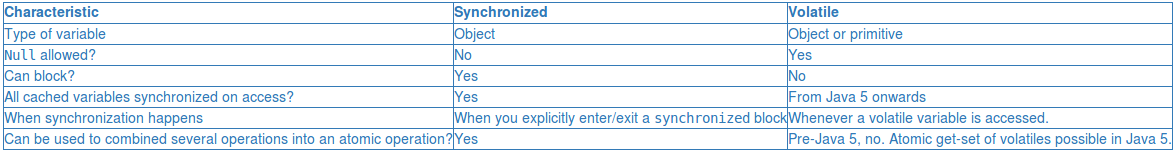
\includegraphics[width = \textwidth]{volvssync.png}
\end{frame}
%-------------------------------------------------------------
\subsubsection{Monitor Locks vs Semaphores}
\begin{frame}
\frametitle{Monitor Locks vs Semaphores}
\begin{itemize}
\item When a {\color{green} thread} enters a {\color{red} synchronized} statement, it owns the {\color{orange} monitor lock} for the object.
\item {\color{orange} monitor locks} restrict access to an object to one single thread. {\color{purple} semaphores} can restrict access to an object to more than one thread.
\end{itemize}
\end{frame}

%----------------------------------------------------------------------------------
\subsection{Thread Interaction 3}
\subsubsection{Wait Notify}
\defverbatim[colored]\waitNotify{
\begin{lstlisting}[style = customjava,basicstyle=\tiny]
if(something)//Check condition before waiting.
	someObject.wait();
//Continues from here after notify
doSomethingElse();
\end{lstlisting}
}
\begin{frame}
\frametitle{Wait Notify}
\begin{itemize}
\item Sometimes want a {\color{orange}thread} to {\color{green}wait} for something in another object to happen before continuing.
\item A {\color{orange} thread} can wait for an object to {\color{red} notify} when something occurs. 
\item This can only be the case if the {\color{orange} thread} owns a {\color{purple} monitor lock} on the object it is waiting to be notified by and therefore must occur in a {\color{magenta} synchronized} block.
\waitNotify
\item This means that the calling object will wait for someObject to call {\color{red} notify} before continuing.
\end{itemize}
\end{frame}

%----------------------------------------------------------------------------------
\subsubsection{wait()}
\begin{frame}
\frametitle{wait()}
\begin{itemize}
\item The calling thread waits for an event to occur in the object called upon. The event could be from another thread or some other operating system event.
\item Throws an Unchecked InterruptException if interrupted and not notified.
\item Can be timed passing a long, similar to sleep.
\item Must be in a synchronized block.
\end{itemize}
\end{frame}

%----------------------------------------------------------------------------------
\subsubsection{notify() and notifyAll()}
\begin{frame}
\frametitle{notify() and notifyAll()}
\begin{itemize}
\item notify()
\begin{itemize}
\item Notifies one random thread. No control in which one.
\end{itemize}
\item notifyAll()
\begin{itemize}
\item Notifies all waiting threads. No reason can be given for the notification.
\end{itemize}
\item Both must be in synchronized blocks.
\end{itemize}

\end{frame}

%---------------------------------------------------------------------------------
\subsubsection{Wait/Notify-Textual Example}
\begin{frame}
\frametitle{Wait/Notify-Textual Example}
\begin{columns}[t]
\column{.5\textwidth}
{\LARGE Producer \\}
Creates goods at random intervals and {\color{red} notifies} consumers.
\begin{enumerate}
\item Sleep for random interval.
\item Make a product.
\item {\color{red} Notify} any thread waiting. 
\end{enumerate}
\column{.5\textwidth}
{\LARGE Consumer \\}
Waits for a producer to make a good, then purchase it.
\begin{enumerate}
\item {\color{blue}Synchronize} on Producer.
\item {\color{green}Wait} for a notification.
\item Buy Product.
\end{enumerate}
\end{columns}
\end{frame}
%----------------------------------------------------------------------------------
\subsubsection{Wait/Notify-Code example}
\defverbatim[colored]\producer{
\begin{lstlisting}[style = customjava,basicstyle=\scriptsize]
public class Producer extends Thread {
	Product good=null;
    int nosGoods = 0;
    public void run() {
    	while(!endOfSimulation()) {
//1) Sleep for random interval.
        	try{
            	sleep((long)(Math.random()*2000));
            }catch(InterruptedException e) {//Should not happen}
            makeGood();
        }
    }
    //Synchronized so only one good can be made at a time.
    public synchronized void makeGood() {
    	if(good == null) {
//2) Make a product.
        	good = new Product(nosGoods);
            nosGoods++;
            System.out.println("Making a good");
//3) Notify waiting thread.
            notify();
        }
    }
}
\end{lstlisting}
}
\begin{frame}
\frametitle{Wait/Notify-Code example - Producer}
\producer
\end{frame}

%----------------------------------------------------------------------------------
\defverbatim[colored]\consumer{
\begin{lstlisting}[style = customjava,basicstyle=\scriptsize]
public class Consumer extends Thread {
	Producer p;
    ArrayList<Product> goods;
    public Consumer(Producer p) {
    	this.p =  p;
        goods = new ArrayList<>();
    }
    public void run() {
    	while(!p.endSimulation()) {
        	if(p.hasGood()) {
//1) Synchronize Producer
            	synchronize(p){
                	try{
//2) Wait for notificaation
                    	p.wait();
                    }catch(InterruptedException e){//Shouldn't happen}
                }
            }
//3) Buy Product.
            goods.add(p.buy());
        }
    }
}
\end{lstlisting}
}
\begin{frame}
\frametitle{Wait/Notify-Code example - Consumer}
\consumer
\end{frame}
%----------------------------------------------------------------------------------
\subsubsection{Wait/Notify Common Problems}
\defverbatim[colored]\locks{
\begin{lstlisting}[style = customjava,basicstyle=\scriptsize]
synchronized (object1);
synchronized (object2) {
	object2.wait();//object2 lock released. object1 still locked
}
\end{lstlisting}
}
\begin{frame}
\frametitle{Wait/Notify Common Problems}
\begin{itemize}
\item You need to check the condition before waiting otherwise risk of never being notified.
\item Waking from wait doesn't mean the condition waiting for has been satisfied, may need a loop of waiting to condition has definitely been satisfied.
\item The timed wait, waits forever if given 0 as a time.
\item Calling wait releases lock on object being waited on, but not on other objects locked by the class:
\locks
\end{itemize}
\end{frame}
%----------------------------------------------------------------------------------
\subsubsection{Wait vs Sleep}
\begin{frame}
\frametitle{Wait vs Sleep}
\begin{itemize}
\item \texttt{Thread.sleep()} is a static method that sends {\color{orange}thread} into the "not runnable" state for a set time.
\item \texttt{lock.wait()} is called on an {\color{green} Object} (lock), {\color{red}not} a {\color{orange}thread}.
\begin{itemize}
\item This causes the current {\color{orange}thread} to wait for the {\color{green}object}. \textbf{It does not cause \texttt{lock} to wait}.
\end{itemize}
\item Before \texttt{lock.wait()} is called, the thread must {\color{blue}synchronize} on the \texttt{lock} object.
\item \texttt{lock.wait()} releases the lock on the object and adds the {\color{orange} thread} to the "wait list" associated with \texttt{lock}.

\item Another {\color{orange} thread} can {\color{blue} synchronize} the same \texttt{lock} object and call \texttt{lock.notify()} that wakes up the original, waiting {\color{orange} thread}.

\item Essentially \texttt{wait()/notify()} is like \texttt{sleep()/interrupt()}, only the active {\color{orange} thread} does not need a direct reference to the sleeping thread, but only to the shared \texttt{lock} object.
\end{itemize} 
\end{frame}

%----------------------------------------------------------------------------------
\subsection{Common Problems with Threads}
\subsubsection{Deadlock}
\begin{frame}
\frametitle{Deadlock}
\begin{itemize}
\item {\color{red} Deadlock} describes a situation where two threads are waiting for each other to finish and never complete.
\item {\color{blue} synchronization} is vital but it can lead to deadlock.
\begin{enumerate}
\item A starts executing and is locked.
\item B starts executing and is locked.
\item A calls B and waits for B to finish
\item B calls A and waits for A to finish
\end{enumerate}
\end{itemize}
\end{frame}
%----------------------------------------------------------------------------------
\subsubsection{Starvation}
\begin{frame}
\frametitle{Starvation}
\begin{itemize}
\item {\color{red} Starvation} is where a {\color{green} thread} is continually denied access to resources and is therefore unable to progress.
\item This happens when "greedy" threads take resources for long periods.
\item Essentially a DDOS on a {\color{green} thread} and can drastically slow down a program.
\item Can be caused by {\color{green} threads} being given a high priority. A deterministic priority queue can cause {\color{red} starvation}.
\end{itemize}
\end{frame}
%----------------------------------------------------------------------------------
\subsubsection{Livelock}
\begin{frame}
\frametitle{Livelock}
\begin{itemize}
\item {\color{green} Threads} often act in response to an action of another thread. 
\item If the other {\color{green} threads} action is also a response to the action of another thread, then {\color{red} livelock} may occur.
\item Unable to make progress.
\item In this case the {\color{green} threads} are not blocked, just responding to each other in a loop.
\item Comparable to the awkward two people passing in a corridor going the same way each time.
\end{itemize}
\end{frame}
%----------------------------------------------------------------------------------
\subsection{Summary}
\begin{frame}
\frametitle{Summary}
\begin{itemize}
\item Made threaded by \texttt{extends Thread} or \texttt{implements Runnable}.
\item run methods run concurrently.
\item Threads claim {\color{red} monitor lock} through keyword {\color{blue} synchronized}.
\item Threads can effect each others run time behaviour through the \texttt{wait/notify \&\& sleep/interrupt. wait/notify} requires {\color{blue} synchronization}.
\item Presents new potential problems
\end{itemize}
\end{frame}
%----------------------------------------------------------------------------------
\begin{frame}
\Huge{\centerline{The End}}
\end{frame}

%----------------------------------------------------------------------------------------

\end{document}